\documentclass{beamer}
%Information
\title{Combination 2: Probability}
\titlegraphic{\hfill
\includegraphics[height=1cm]{orange.png}}
\institute{Youth STEM Academy}
\author{Erzhuo Wang}
\date{\today}
%Theme
\usetheme[block=fill, sectionpage=none]{metropolis}
\useoutertheme{infolines}
\useinnertheme{metropolis}
\setbeamertemplate{blocks}[rounded][shadow=false]
\setbeamertemplate{items}[ball]
\setbeamertemplate{sections/subsections in toc}[ball]
\setbeamertemplate{headline}{}
\logo{YSA}
\usecolortheme{custom}
%\usetheme{Madrid}
%\usetheme{Heverlee}

%Setting
\usepackage[UTF8,noindent]{ctexcap}
\ctexset{today=old}
\theoremstyle{definition}
\newtheorem{defn}{Definition}[section]
\newtheorem{coro}[defn]{Corollary}
\newtheorem{theo}[defn]{Theorem}
\newtheorem{exer}[defn]{Exercise}
\newtheorem{rema}[defn]{Remark}
\newtheorem{lem}[defn]{Lemma}
\newtheorem{prop}[defn]{Proposition}
\newtheorem{nota}[defn]{Notation}
\newtheorem{exam}[defn]{Example}
\newtheorem{ques}[defn]{Question}

\newenvironment{prooff}{{\noindent\it\textcolor{cyan!40!black}{Proof}:}\,}{\par}
\newenvironment{proofff}{{\noindent\it\textcolor{cyan!40!black}{Proof of the lemma}:}\,}{\qed \par}
\newcommand{\bbrace}[1]{\left\{ #1 \right\} }
\newcommand{\bb}[1]{\mathbb{#1}}
\newcommand{\p}{^{\prime}}
\renewcommand{\mod}[1]{(\text{mod}\,#1)}
\newcommand{\blue}[1]{\textcolor{blue}{#1}}
\newcommand{\spec}[1]{\text{Spec}({#1})}
\newcommand{\rarr}[1]{\xrightarrow{#1}}
\newcommand{\larr}[1]{\xleftarrow{#1}}
\newcommand{\emptyy}{\underline{\quad}}
\newenvironment{enu}{\begin{enumerate}[(1)]}{\end{enumerate}}
%ctrl+点击文本返回代码  选中代码 ctrl+alt+j 为代码查找文本

\begin{document}
\begin{frame}
    \titlepage
\end{frame}
\begin{frame}{Introduction}
    这节课我们来处理与概率有关的问题, 这类的问题的一个特点是没有固定的思路, 需要灵活运用知识点。 
    
    但是一些与概率有关的经典问题和思想我们需要进行讨论, 如条件概率的思想以及二项分布问题。
\end{frame}
\begin{frame}{Definition of Probability}
    如果样本空间的总量有限, 且每个样本空间的子事件概率相同, 则某个事件发生的概率可以理解为
    $$
      \frac{\text{该事件发生的情况总数}}{\text{总事件个数}}
    $$
    \begin{ques}
        Two different numbers are randomly selected from $-2,-1,0,3,4,5$ and multiplied together. What is the probablity
    that the product is $0$?
    从$-2,-1,0,3,4,5$中随机选择两个不同的数字并相乘, 为0的概率是多少?
    \end{ques}
    如果子事件发生概率不同, 某个事件的概率应该为该事件的所有子事件的概率分别相加。
\end{frame}
\section{Counting Principle}
\begin{frame}{Binomial Distribution(二项分布)}
    A typical problem about binomial distribution is the coin toss.
    Consider a coin of uneven texture with a probability of $p\in (0,1)$ for heads and a probability of $1-p$ for tails.
    Find the probability of $k$ heads after flipping $n$ times.

    与二项分布有关的问题中最经典的问题为抛硬币问, 考虑一枚质地不均匀的硬币, 每次抛该硬币得到正面的概率为$p\in (0,1)$, 反面的概率为$1-p$.
    求抛$n$次后$k$次正面的概率.
\end{frame}
\begin{frame}{Binomial Distribution(二项分布)}
    \begin{theo}
        Probability of $k$ heads after flipping $n$ times is $\binom{n}{k}p^k(1-p)^{n-k}$
    \end{theo}
    \begin{exam}
        A fair coin is tossed ten times. Find the probability of getting six heads and four tails.

        质地均匀的硬币投十次, 求反面出现四次的概率.
    \end{exam}
\end{frame}
\begin{frame}{Special Dice (AMC 8, 2018-18)}
    \begin{ques}
        The faces of a "special dice" are numbered $1,2,3,5,7$, and 8. When two "special dice" are tossed, what is the
        probability that their sum will be an even number?

        一种特殊的骰子面上的数字为$1,2,3,5,7,8$, 投两个这样的筛子, 得到的数字加起来为偶数的概率是多少?
    \end{ques}
    \begin{ques}
        Replace "two special dice are tossed" in above Question by "three special dice are tossed".

        将上题投两个改成投三个。
    \end{ques}
\end{frame}
% \begin{frame}{Solution}
%     \begin{prooff}

%     \end{prooff}
% \end{frame}
% \begin{frame}{Sample Space(样本空间)}
%     The sample space $S$ is the set of all possible outcomes. For example,
%     if the experiment is that of flipping a fair coin three times,
%     where each flip comes up heads $(\mathbf{H})$ or tails $(\mathbf{T})$,
%     then the sample space is $S=$ $\{H H H, H H T, H T H, H T T, T H H, T H T, T T H, T T T\}$.
%     A subset of the sample space is called an event.
%     For example, when flipping a coin three times, we may be interested in the event that exactly two heads are seen,
%     so the event is $E=\{H H T, H T H, T H H\}$.
% \end{frame}
% A probability function, $\mathbb{P}$, assigns to each event a real number and obeys the following rules:

% (1): For each event $E, \mathbb{P}(E) \geq 0$.

% (2): $\mathbb{P}(S)=1$.

% (3): If $E_1, E_2, E_3, \ldots$ is a sequence(always finite sequence in our courses)
% of pairwise disjoint events, then the probability of their union is the sum of their probabilities,
% that is,
% $$
%     \mathbb{P}\left(\bigcup E_j\right)=\sum \mathbb{P}\left(E_j\right)
% $$.
\begin{frame}{Conditional Probability(条件概率)}
    We denote the probability that event $A$ occurs under the condition $B$ by $\mathbb{P}(A|B)$.

    \begin{theo}[Conditional probability of $A$ given $B$]
        \begin{equation*}
            \mathbb{P}(A|B)=\frac{\bb{P}(A\cap B)}{\bb{P}(B)}
        \end{equation*}
    \end{theo}

    \begin{exam}
        Flip a fair coin three times. Find the probability that the first flip comes out heads given that there aree exactly $2$ heads flipped.

        抛一枚质地均匀的硬币两次, 求在有共两次正面的条件下第一次为正面的概率.
    \end{exam}
\end{frame}
\begin{frame}
\begin{theo}[Law of total probability(全概率公式)]
    \begin{equation*}
        \bb{P}(A)=\bb{P}(A|B)\bb{P}(B)+\bb{P}(A|B^c)\bb{P}(B^c)
    \end{equation*}
\end{theo}
\begin{exam} 
    用全概率公式证明: 任意抛$n$次均匀的硬币, 正面朝上的次数是偶数(或奇数)的概率为$1/2$.
\end{exam}
\end{frame}
\begin{frame}{Jumping Cricket(AMC 8, 2022-25)}
    A cricket randomly hops between $4$ leaves,
    on each turn hopping to one of the other $3$ leaves with equal probability. After $4$ hops what is the probability that the cricket has returned to the leaf where it started?
    \begin{figure}
        \centering
        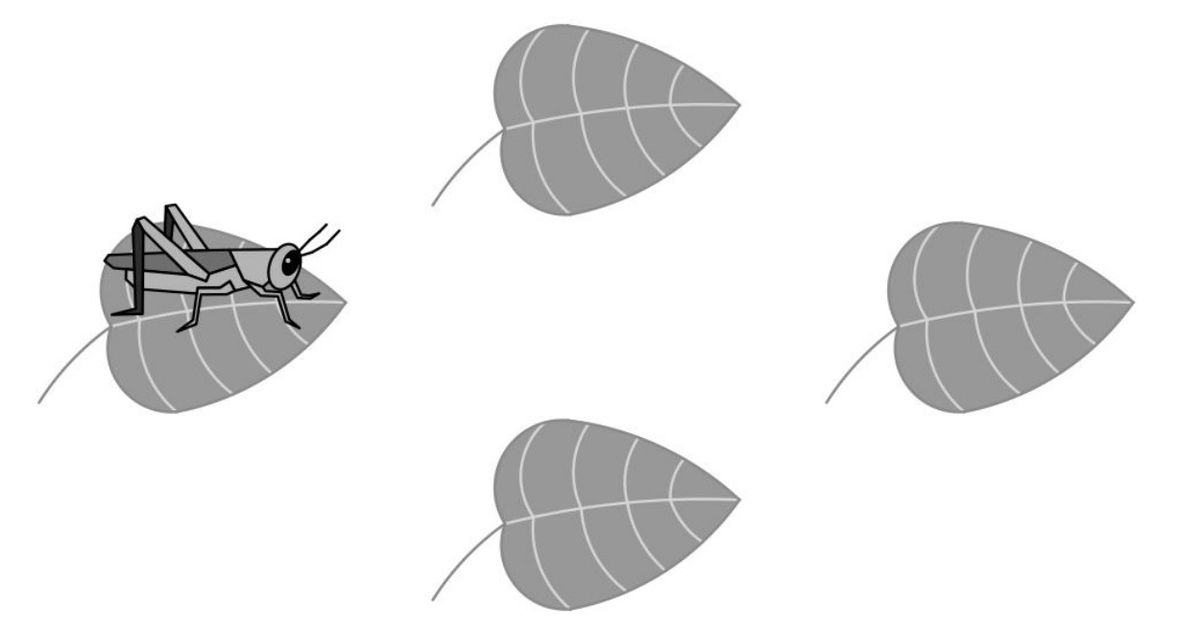
\includegraphics[width=0.5\textwidth]{AMC8-2022-25.jpg}
    \end{figure}
\end{frame}
\begin{frame}{跳跃的蟋蟀(AMC 8, 2022-25)}
    一个蟋蟀随意的在四片叶子上跳跃, 每次等概率得跳向其他三片叶子之一, 求蟋蟀跳四次后返回最初这片叶子的概率.
    \begin{figure}
        \centering
        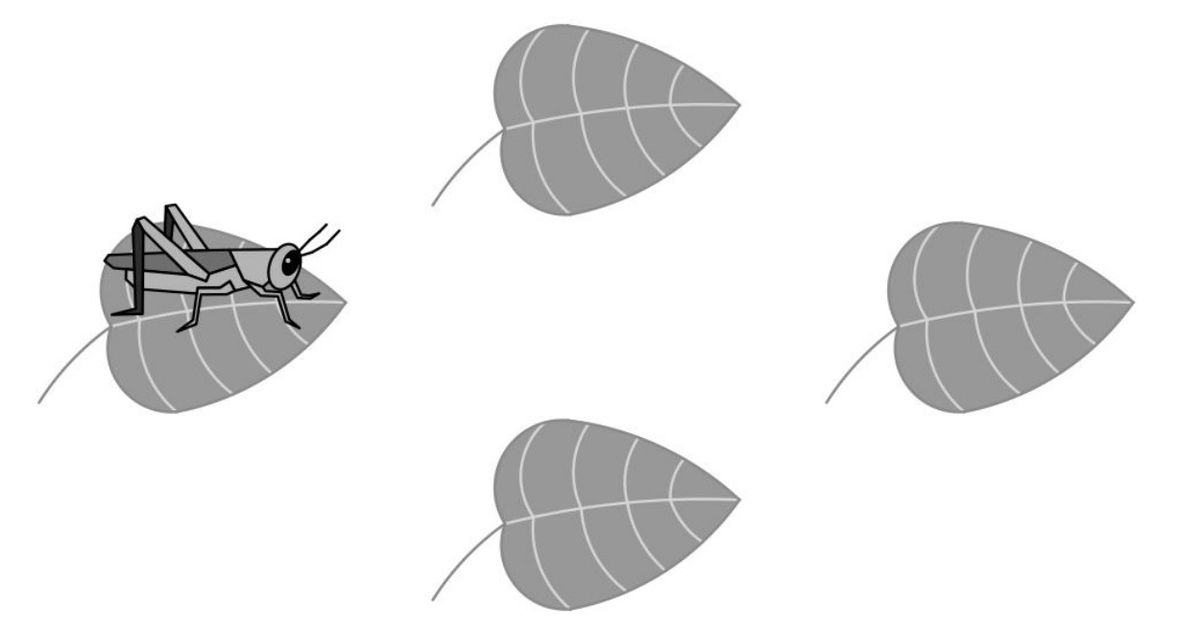
\includegraphics[width=0.5\textwidth]{AMC8-2022-25.jpg}
    \end{figure}
\end{frame}
\begin{frame}{Solution}
    Assume the cricket start from the leaf $A$.
    Let $\bb{P}(A_n)$ be the probability that the cricket returns to the leaf after $n$ times jumping. $\bb{P}(B_n)$ be the
    probability that the cricket doesn't retrun to the leaf after $n$ times jumping.
    By Law of total probability,
    \begin{align*}
        \bb{P}(A_n) & =\bb{P}(A_n|B_{n-1})\bb{P}(B_{n-1})+\bb{P}(A_n|B_{n-1}^c)\bb{P}(B_{n-1}^c)=\frac{1}{3}\bb{P}(B_{n-1}) \\
                    & =\frac{1}{3}(1-\bb{P}(A_{n-1}))
    \end{align*}
    Since $ \bb{P}(A_1)=0$, it's easy to calculate $\bb{P}(A_4)$.

\end{frame}
\begin{frame}{Seats Distributing(分配座位)}
    \begin{ques}
        A small airplane has $4$ rows of seats with $3$ seats in each row.
        Eight passengers have boarded the plane and are distributed randomly among the seats. A married couple is next to board. What is the probability there will be $2$ adjacent seats in the same row for the couple?

        一辆小飞机排布有四行三列座位, 8个乘客随机地坐在这12个座位上, 求这八个人坐完后还可以剩下一对同一行的相邻座位的概率?
    \end{ques}
\end{frame}
\begin{frame}{Solution}
    \begin{prooff}
        There are $\binom{12}{8}=495$ total ways to distribute the passengers. It suffices to count the number of passenger arrangements such that the couple cannot sit anywhere. Consider the partitions of $8$ among the rows of $3$ seats.
        We have third pattern of partition: $(3,3,1,1),(3,2,2,1),(2,2,2,2)$

        For the first partition, there are $6$ ways to permute the partition. Now the rows with exactly 1 passenger must be in the middle, so this case generates 6 cases.

        For the second partition, there are $12$ ways to permute the partition. For rows with 2 passengers, there are $\binom{3}{2}=3$ ways to arrange them in the row so that the couple cannot sit there. The row with 1 passenger must be in the middle. We obtain $12 \cdot 3^2=108$ cases.
    \end{prooff}
\end{frame}
For the third partition, rows with 2 passengers can be arranged in 3 ways, so we obtain $3^4=81$ cases.

Collectively, we obtain a grand total of $6 + 108 + 81 = 195$ cases. The final probability is $\frac{20}{33}$.
\begin{frame}{Octagon(AMC8 2018-23)}
    From a regular octagon, a triangle is formed by connecting three randomly chosen vertices of the octagon. What is the probability that at least one of the sides of the triangle is also a side of the octagon?
    \begin{figure}
        \centering
        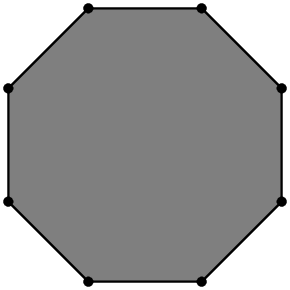
\includegraphics[width=0.3\textwidth]{triangle.png}
    \end{figure}

    (A) $\frac{2}{7}$ (B) $\frac{5}{42}$ (C) $\frac{11}{14}$ (D) $\frac{5}{7}$ (E) $\frac{6}{7}$
\end{frame}
\begin{frame}{Exercise}
    
\begin{ques}[AMC8 2017-20]
    An integer $x$ satisfying $1000\le x\le 9999$, is chosen at random. What is the probability that it is an odd integer whose digits are all distinct?
    
    (A) $\frac{14}{75}$ (B) $\frac{56}{225}$ (C) $\frac{107}{400}$ (D) $\frac{7}{25}$ (E) $\frac{9}{25}$
\end{ques}
\begin{ques}[AMC 8 2016-21]
    A top hat contains 3 red chips and 2 green chips. Chips are drawn randomly, one at a time without replacement, until all 3 of the reds are drawn or until both green chips are drawn. What is the probability that the 3 reds are drawn?
    
    (A) $\frac{3}{10}$ (B) $\frac{2}{5}$ (C) $\frac{1}{2}$ (D) $\frac{3}{5}$ (E) $\frac{7}{10}$
\end{ques}

\end{frame}


\begin{frame}{Homework}
    \begin{ques}
        Coin $A$ is flipped three times and coin $B$ is flipped four times.

        (1): Find the probability that both of these coins have two heads.

        (2): Find the probability that these two coins have the same number of heads.

        抛质地均匀的硬币$A$共$3$次, $B$共$4$次,

        (1): 求这两个硬币正面次数均为两次的概率的概率.

        (2): 求这两个硬币正面次数相同的概率.
    \end{ques}
\end{frame}
% \begin{frame}{Homework}
%     \begin{ques}
%         Suppose that a box contains $3$ red balls, $2$ blue balls, and $1$ white ball while a second
%         box contains $3$ white balls, $2$ blue balls, and $1$ red ball. If you randomly select a box, and randomly select two balls without replacement from
%         that the box, what is the probablity that you selected the first box given that you selected one red ball and one blue ball?
%         一个盒子里有三红球, 两蓝球, 一白球, 第二个盒子有三白球, 两蓝球, 一红球. 随机选一个盒子并从该盒子里随机拿两个. 
%         求抽到一红一蓝球的条件下, 选择第一个盒子的概率.
%     \end{ques}
% \end{frame}
\begin{frame}{Homework}
    Each square in a $3 \times 3$ grid is randomly filled with one of the 4 gray and white tiles shown below on the right.
\begin{figure}
    \centering
    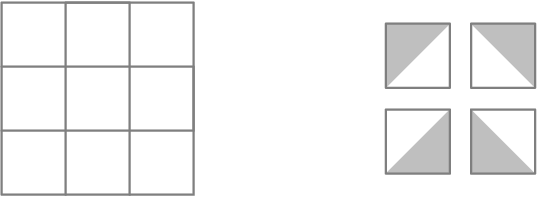
\includegraphics[width=0.5\textwidth]{grid.png}
\end{figure}
What is the probability that the tiling will contain a large gray diamond in one of the smaller $2 \times 2$ grids? Below is an example of such tiling.
\begin{figure}
    \centering
    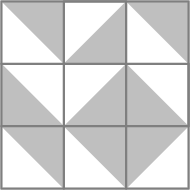
\includegraphics[width=0.2\textwidth]{grid2.png}
\end{figure}
\end{frame}
(A) $1/2024$ (B) $1/256$ (C) $1/64$ (D) $1/16$ (E) $1/4$

\begin{ques}
    在海滩上,50个人戴着太阳镜,35个人戴着帽子。有些人既戴太阳镜又戴帽子。
    如果随机选择一个戴帽子的人,
    这个人也戴太阳镜的概率是$\frac{2}{5}$. 如果随机选择一个戴太阳镜的人,这个人也戴帽子的概率是多少?
\end{ques}
\begin{ques}
    A box contains exactly five chips, three red and two white. Chips are randomly removed one at a time without
    replacement until all the red chips are drawn or all the white chips are drawn. What is the probability that the last chip drawn is white?

    一个盒子里正好有5个筹码,3个红牌,2个白牌。每次随机取出一张筹码,直到所有红牌或白牌都被取出为止。最后一张牌是白色的概率是多少?
\end{ques}




\end{document}